\documentclass[10pt]{article}
\usepackage[margin=0.7in]{geometry}
\usepackage{booktabs,graphicx,amssymb,longtable,multirow}
\usepackage[T1]{fontenc}
\usepackage{placeins}
\usepackage{xcolor}
\usepackage[colorlinks=true,linkcolor=blue!50!black]{hyperref}
\newcommand{\rqsection}[2]{\FloatBarrier\clearpage\section*{#1}\noindent\emph{#2}\par\medskip}
\newcommand{\addresses}[1]{\noindent\textbf{Addresses:} #1\par\medskip}
\setcounter{topnumber}{3}\renewcommand{\topfraction}{0.95}\setcounter{totalnumber}{4}\renewcommand{\textfraction}{0.02}
\renewcommand{\floatpagefraction}{0.9}\renewcommand{\dbltopfraction}{0.95}\renewcommand{\dblfloatpagefraction}{0.9}
\title{Tree kernels on BigCloneBench: revised results (all eligible queries)}
\date{exp\_v3\_all\_queries, \today}
\begin{document}
\maketitle

\noindent This document collects the tables and figures of the revised evaluation, as planned in
\texttt{revision\_plan.md}. The setting, metrics and statistics are described once, in the section \emph{Setup};
captions only say what a table or figure shows.

\medskip
\noindent\begin{tabular}{@{}ll@{}}
\toprule
Section & Reviewer comments \\
\midrule
RQ1, RQ2 & R1-C1a (all queries), R1-C2a (fine-tuned CodeBERT), R2-C5 (effect sizes, $p$-values) \\
RQ3 & R2-C4 (no thresholds: LOC quartiles, McCabe bins), R1-C1a \\
RQ4 & R2-C5 (hybrid effect sizes and metric-level $p$-values), R1-C1a \\
Kernel hyper-parameters & R1-C1b ($\lambda$, $\mu$, terminal factor) \\
Label noise & R1-C3 (BigCloneBench label noise) \\
Diagnostics & R1-C4 (tree depth, nodes, branching) \\
\bottomrule
\end{tabular}

\FloatBarrier\clearpage
\section*{Setup}

%\paragraph{Corpus.} BigCloneBench's true positives plus its 58,103 false positives: 72,782 Java methods. Every query is ranked against the whole corpus. A false positive counts as non-relevant, except a whitespace-identical copy of the query, which is removed from that query's ranking (BigCloneBench evidently mislabelled it).

%\paragraph{Queries.} Every eligible true positive is a query (R1-C1a): the 14,679 true positives minus the 50 tuning queries and the 42 methods whose functionalities span CodeBERT folds, i.e.\ 14,587. No sampling is involved.
%14,780 tps in bcb but 101 had overflow on KeLP. 219 fps also overflew but not relevant to queries.


\paragraph{Confidence intervals and tests.} Queries of the same functionality implement the same task, look alike
and share relevant methods, so they are not independent. To compute confidence intervals we resample 43 functionalities (not individual queries) 10,000 times with replacement. Each resample keeps all queries of each drawn functionality. %If a query appears in several functionalities is considered a part of the lowest-numbered functionality. 
Comparisons are paired i.e., both methods are scored on the same queries in every resample. Since all eligible queries are evaluated, the intervals do not describe sampling of queries; they show how far a result would change on a different set of tasks.
\begin{itemize}
\item \emph{Tested comparisons}: MAP is the primary metric and the only one tested. In RQ1 (for each clone type and
for the mean of the five types) and in RQ2, the 9 comparisons are the three kernels against each other and each
kernel against BM25 and against fine-tuned CodeBERT. In RQ4, the 9 comparisons per measure are each hybrid against
its kernel's full ranking, BM25 and fine-tuned CodeBERT.
\item \emph{Bonferroni-adjusted CI}: to account for the multiple comparisons, each CI is widened to the level
$1 - 0.05/m$ for a family of $m$ comparisons (99.4\% for 9): the middle 99.4\% of the 10,000
resampled differences. A difference is significant when its adjusted CI excludes 0.
\item \emph{Effect size $A_{12}$} (paired Vargha--Delaney): the share of queries on which A scores higher than B, plus
half the ties; 0.5 = no difference. Labels: negligible $<$ 0.56, small $\geq$ 0.56, medium $\geq$ 0.64, large $\geq$
0.71 (and symmetrically below 0.5).
\item All other results (the other metrics, comparisons between the baselines, RQ3, label noise and the diagnostics)
are reported as values over all eligible queries, without CIs or tests.
\end{itemize}


%\paragraph{Label noise.} Every method is re-evaluated on the same rankings under two alternative labellings.
%\emph{Type-2 copies ignored}: additionally removed from a query's ranking is every method that is a Type-2 copy of the
%query (identical token sequence after replacing identifiers by one placeholder and literals by another, comments and
%whitespace removed) but is not labelled as sharing its functionality: 428 query--false positive pairs (360 of them
%already ignored as whitespace-identical) and 4 true positives of other functionalities, affecting 178 queries.
%\emph{False positives removed}: all 58,103 false positives are removed from every ranking, as if they had never been
%judged.

\rqsection{RQ1. Syntactic similarity}{How well do tree kernels retrieve syntactic clones of each type (T1, T2, VST3, ST3, MT3), compared with BM25 and CodeBERT?}
\addresses{R1-C1a, R1-C2a, R2-C5.}
\begin{table*}[!htbp]
\centering
\caption{Syntactic clones per clone type, every eligible query. MAP: $^{+}$/$^{-}$ significantly better/worse than BM25; $^{\uparrow}$/$^{\downarrow}$: tree kernel significantly better/worse than fine-tuned CodeBERT (Bonferroni-adjusted CI excludes 0). Best value per block and column in bold. Test results are shown in Figure~\ref{fig:rq1}.}
\label{tab:rq1}
\footnotesize
\setlength{\tabcolsep}{4pt}
\begin{tabular}{l|lcccc}
\toprule
Clone type & Method & nP@5 & nP@10 & MRR & MAP \\
\midrule
\multirow{6}{*}{T1} & STK & \textbf{1.000} & \textbf{1.000} & \textbf{1.000} & \textbf{1.000} \\
 & SSTK & \textbf{1.000} & \textbf{1.000} & \textbf{1.000} & \textbf{1.000} \\
 & PTK & \textbf{1.000} & \textbf{1.000} & \textbf{1.000} & \textbf{1.000} \\
 & BM25 & \textbf{1.000} & \textbf{1.000} & 0.999 & 0.999 \\
 & CodeBERT zs & 0.999 & 0.999 & 0.999 & 0.999 \\
 & CodeBERT ft & \textbf{1.000} & \textbf{1.000} & \textbf{1.000} & \textbf{1.000} \\
\midrule
\multirow{6}{*}{T2} & STK & 0.999 & 0.999 & \textbf{0.997} & 0.995$^{+\uparrow}$ \\
 & SSTK & 0.999 & 0.999 & \textbf{0.997} & 0.996$^{+\uparrow}$ \\
 & PTK & \textbf{1.000} & \textbf{1.000} & \textbf{0.997} & \textbf{0.997}$^{+\uparrow}$ \\
 & BM25 & 0.912 & 0.931 & 0.907 & 0.886 \\
 & CodeBERT zs & 0.983 & 0.983 & 0.977 & 0.970 \\
 & CodeBERT ft & 0.973 & 0.978 & 0.963 & 0.958 \\
\midrule
\multirow{6}{*}{VST3} & STK & \textbf{0.994} & \textbf{0.998} & 0.992 & 0.990$^{+\uparrow}$ \\
 & SSTK & \textbf{0.994} & 0.997 & 0.993 & \textbf{0.991}$^{+\uparrow}$ \\
 & PTK & 0.993 & 0.995 & \textbf{0.994} & 0.989$^{+\uparrow}$ \\
 & BM25 & 0.942 & 0.947 & 0.947 & 0.934 \\
 & CodeBERT zs & 0.969 & 0.974 & 0.963 & 0.959 \\
 & CodeBERT ft & 0.967 & 0.972 & 0.960 & 0.955 \\
\midrule
\multirow{6}{*}{ST3} & STK & 0.927 & 0.931 & 0.938 & 0.893$^{+\uparrow}$ \\
 & SSTK & 0.936 & 0.938 & \textbf{0.942} & 0.902$^{+\uparrow}$ \\
 & PTK & \textbf{0.939} & \textbf{0.945} & 0.940 & \textbf{0.912}$^{+\uparrow}$ \\
 & BM25 & 0.810 & 0.811 & 0.838 & 0.771 \\
 & CodeBERT zs & 0.833 & 0.850 & 0.865 & 0.794 \\
 & CodeBERT ft & 0.828 & 0.836 & 0.853 & 0.789 \\
\midrule
\multirow{6}{*}{MT3} & STK & 0.629 & 0.618 & 0.735 & 0.500 \\
 & SSTK & 0.640 & 0.624 & 0.740 & 0.508 \\
 & PTK & \textbf{0.647} & \textbf{0.638} & \textbf{0.754} & \textbf{0.537} \\
 & BM25 & 0.545 & 0.545 & 0.649 & 0.453 \\
 & CodeBERT zs & 0.521 & 0.517 & 0.648 & 0.392 \\
 & CodeBERT ft & 0.599 & 0.593 & 0.694 & 0.491 \\
\midrule
\multirow{6}{*}{\begin{tabular}{@{}l@{}}Mean of\\5 types\end{tabular}} & STK & 0.910 & 0.909 & 0.932 & 0.876$^{+}$ \\
 & SSTK & 0.914 & 0.912 & 0.934 & 0.879$^{+}$ \\
 & PTK & \textbf{0.916} & \textbf{0.916} & \textbf{0.937} & \textbf{0.887}$^{+}$ \\
 & BM25 & 0.842 & 0.847 & 0.868 & 0.808 \\
 & CodeBERT zs & 0.861 & 0.865 & 0.890 & 0.823 \\
 & CodeBERT ft & 0.873 & 0.876 & 0.894 & 0.839 \\
\bottomrule
\end{tabular}
\end{table*}

\begin{figure*}[!htbp]\centering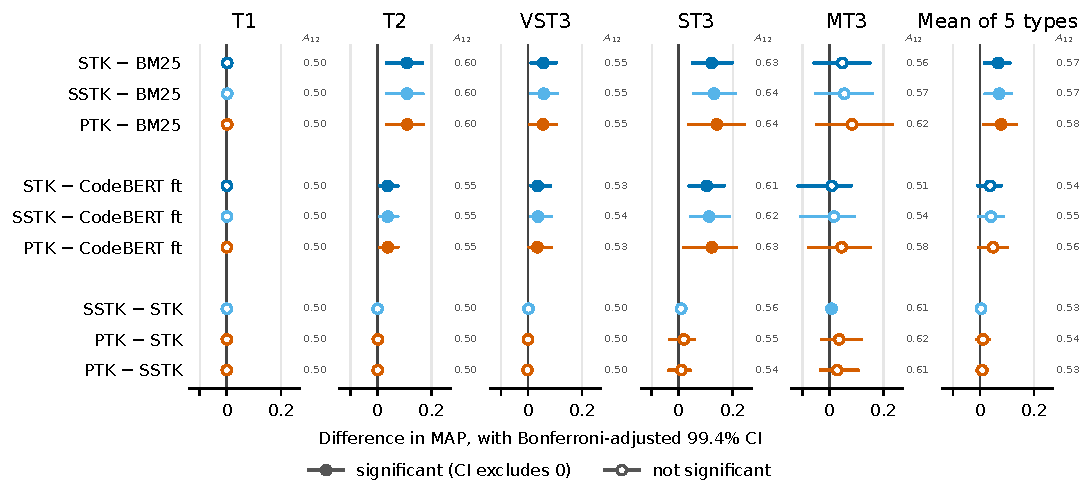
\includegraphics[width=\textwidth]{figures/rq1_forest}\caption{RQ1 tests on MAP: difference A $-$ B with Bonferroni-adjusted 99.4\% CI (9 comparisons per clone type) and effect size $A_{12}$ (right of each panel). Filled: the CI excludes 0.}\label{fig:rq1}\end{figure*}

%What it shows better than Table 2
%- All the RQ1 conclusions at a glance: T1 is flat at 0, T2, VST3 and ST3 are filled for both baselines, and MT3 has wide CIs that cross 0.
%- The size of the uncertainty, which grows from T2 to MT3.
%- The lead over CodeBERT ft on the mean of types: the CIs just cross 0.

Table~\ref{tab:rq1} shows the results per clone type for the three tree kernel variants, BM25, and
CodeBERT in zero-shot and fine-tuned settings, on every eligible query from BigCloneBench.
Figure~\ref{fig:rq1} shows the significance tests of the kernel comparison with BM25, with fine-tuned CodeBERT and with the other kernels. MAP is the primary metric and the only one tested. A marker on a MAP value in Table~\ref{tab:rq1} indicates a significant comparison with a baseline,
i.e.\ the corresponding Bonferroni-adjusted CI in Figure~\ref{fig:rq1} excludes 0. Comparisons among the baselines and with zero-shot CodeBERT are not tested, so the baseline rows carry no markers.

On T1, every method scores nearly 1.0. On T2, VST3 and ST3, all three kernels perform significantly
better than both BM25 and fine-tuned CodeBERT. On MT3, no kernel differs significantly from either
baseline, as their CIs span 0. Across the mean of the five types, the kernels significantly beat
BM25, but their lead over fine-tuned CodeBERT is not significant. Among the kernels, the only
significant difference is SSTK over STK on MT3, and it is very small (+0.008 MAP).


\rqsection{RQ2. Functional similarity}{What is the performance of three tree kernels for functionally similar source code retrieval?}
\addresses{R1-C1a, R1-C2a, R2-C5; R1-C3 for the label quality of WT3/T4 pairs (section Label noise).}
\begin{table*}[!htbp]
\centering
\caption{Functional similarity on every eligible query, and mean runtime cost. Best metric value per block and column in bold. MAP: $^{+}$/$^{-}$ significantly better/worse than BM25; $^{\uparrow}$/$^{\downarrow}$: tree kernel significantly better/worse than fine-tuned CodeBERT (Bonferroni-adjusted CI excludes 0). Corresponding test results are in Figure~\ref{fig:rq2}. One-off cost is paid once, not per query.}
\label{tab:rq2}
\footnotesize
\setlength{\tabcolsep}{4pt}
\begin{tabular}{lcccc||rrr}
\toprule
Method & nP@5 & nP@10 & MRR & MAP & Per query (s) & All queries (h) & One-off (s) \\
\midrule
STK & 0.657 & 0.600 & 0.821 & 0.183$^{-\downarrow}$ & 6.73 & 27.3 & 88 \\
SSTK & 0.654 & 0.600 & 0.820 & 0.182$^{-\downarrow}$ & 6.98 & 28.3 & 83 \\
PTK & 0.617 & 0.562 & 0.789 & 0.165$^{-\downarrow}$ & 15.51 & 62.8 & 116 \\
\cmidrule(lr){1-8}
BM25 & 0.743 & 0.704 & \textbf{0.875} & \textbf{0.443} & 0.70 & 2.8 & 14 \\
CodeBERT zs & 0.627 & 0.575 & 0.798 & 0.144 & 0.41 & 1.7 & 22,344 \\
CodeBERT ft & \textbf{0.753} & \textbf{0.724} & 0.868 & 0.434 & 0.41 & 1.7 & see text \\
\bottomrule
\end{tabular}
\end{table*}

\begin{figure}[!htbp]\centering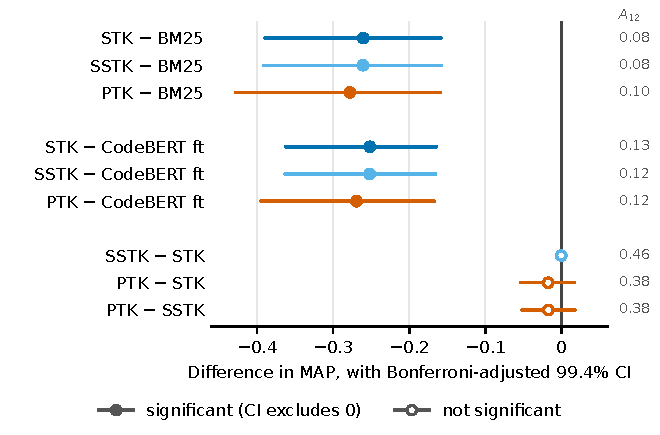
\includegraphics[width=0.62\textwidth]{figures/rq2_forest}\caption{Tests on MAP: difference A $-$ B with Bonferroni-adjusted 99.4\% CI (9 comparisons) and effect size $A_{12}$ (right). Filled: the CI excludes 0.}\label{fig:rq2}\end{figure}

\paragraph{Runtime}

Timing was measured on functional queries against the full corpus of 72,782 methods,
on one thread. One-off costs are paid once, not per query: for the tree kernels, parsing the methods, building the trees, reading them and computing the corpus self-similarities; for BM25, building the Elasticsearch index, which uses Elasticsearch's own threads; for CodeBERT, loading the model and encoding the corpus, estimated from 2,000 random methods encoded one at a time. Fine-tuned CodeBERT has the same per-query cost as zero-shot; in addition, each of its 5 fold models is fine-tuned (3.7--6.2 h per model) and encodes the corpus (2.8--4.0 h per model), measured on 14 threads.





\rqsection{RQ3. Size and complexity}{Do the techniques' results, and the differences between them, depend on the size (lines of code) or the cyclomatic complexity of the query?}
\addresses{R2-C4 (no size or complexity thresholds; McCabe $>$ 10 as sensitivity), R1-C1a.}
\begin{table*}[!htbp]
\centering
\caption{RQ3: MAP per quartile of the query's lines of code and per bin of its McCabe complexity. Syntactic similarity: mean of the five clone types. Last rows: (type-)queries per group.}
\label{tab:rq3}
\footnotesize
\setlength{\tabcolsep}{3.5pt}
\begin{tabular}{lcccc|ccccc}
\toprule
 & \multicolumn{4}{c|}{Lines of code (quartile)} & \multicolumn{5}{c}{McCabe} \\
Method & Q1 (3--13) & Q2 (14--21) & Q3 (22--35) & Q4 (36--433) & 1 & 2--3 & 4--5 & 6--10 & >10 \\
\midrule
\multicolumn{10}{l}{\emph{Syntactic similarity, mean of the five types}} \\
\quad STK & 0.875 & 0.860 & 0.872 & 0.925 & 0.891 & 0.855 & 0.881 & \textbf{0.882} & 0.935 \\
\quad SSTK & 0.881 & 0.865 & 0.875 & 0.924 & 0.895 & 0.861 & 0.885 & \textbf{0.882} & 0.936 \\
\quad PTK & \textbf{0.912} & \textbf{0.881} & 0.870 & 0.854 & \textbf{0.901} & \textbf{0.889} & \textbf{0.897} & 0.876 & 0.829 \\
\cmidrule(lr){1-10}
\quad BM25 & 0.715 & 0.820 & \textbf{0.881} & \textbf{0.942} & 0.722 & 0.758 & 0.825 & 0.881 & \textbf{0.961} \\
\quad CodeBERT zs & 0.823 & 0.788 & 0.818 & 0.890 & 0.775 & 0.808 & 0.820 & 0.844 & 0.905 \\
\quad CodeBERT ft & 0.829 & 0.816 & 0.842 & 0.889 & 0.799 & 0.820 & 0.850 & 0.847 & 0.911 \\
\quad Queries & 7,327 & 4,859 & 4,032 & 2,891 & 1,917 & 7,001 & 5,694 & 3,019 & 1,478 \\
\midrule
\multicolumn{10}{l}{\emph{Functional similarity}} \\
\quad STK & 0.323 & 0.182 & 0.123 & 0.080 & 0.196 & 0.244 & 0.215 & 0.114 & 0.079 \\
\quad SSTK & 0.322 & 0.180 & 0.123 & 0.081 & 0.196 & 0.244 & 0.215 & 0.113 & 0.079 \\
\quad PTK & 0.301 & 0.167 & 0.102 & 0.069 & 0.133 & 0.219 & 0.210 & 0.106 & 0.071 \\
\cmidrule(lr){1-10}
\quad BM25 & \textbf{0.557} & 0.451 & \textbf{0.424} & \textbf{0.322} & \textbf{0.470} & \textbf{0.530} & 0.462 & 0.380 & \textbf{0.289} \\
\quad CodeBERT zs & 0.235 & 0.132 & 0.108 & 0.087 & 0.097 & 0.184 & 0.181 & 0.104 & 0.080 \\
\quad CodeBERT ft & 0.546 & \textbf{0.462} & 0.404 & 0.307 & 0.399 & 0.511 & \textbf{0.471} & \textbf{0.392} & 0.278 \\
\quad Queries & 4,071 & 3,559 & 3,462 & 3,495 & 1,373 & 4,399 & 3,794 & 3,142 & 1,878 \\
\bottomrule
\end{tabular}
\end{table*}

\begin{table}[!htbp]
\centering
\caption{RQ3, McCabe's threshold: MAP of queries with McCabe $\leq$ 10 and $>$ 10, and the difference.}
\label{tab:mccabe10}
\footnotesize
\setlength{\tabcolsep}{3.5pt}
\begin{tabular}{lccc}
\toprule
Method & $\leq$ 10 & $>$ 10 & $>$10 $-$ $\leq$10 \\
\midrule
\multicolumn{4}{l}{\emph{Syntactic similarity, mean of the five types}} \\
\quad STK & 0.873 & 0.935 & +0.063 \\
\quad SSTK & 0.877 & 0.936 & +0.059 \\
\quad PTK & 0.891 & 0.829 & -0.063 \\
\quad BM25 & 0.799 & 0.961 & +0.162 \\
\quad CodeBERT zs & 0.818 & 0.905 & +0.088 \\
\quad CodeBERT ft & 0.834 & 0.911 & +0.077 \\
\midrule
\multicolumn{4}{l}{\emph{Functional similarity}} \\
\quad STK & 0.198 & 0.079 & -0.119 \\
\quad SSTK & 0.198 & 0.079 & -0.118 \\
\quad PTK & 0.179 & 0.071 & -0.108 \\
\quad BM25 & 0.466 & 0.289 & -0.177 \\
\quad CodeBERT zs & 0.154 & 0.080 & -0.074 \\
\quad CodeBERT ft & 0.458 & 0.278 & -0.180 \\
\bottomrule
\end{tabular}
\end{table}

\begin{figure*}[!htbp]\centering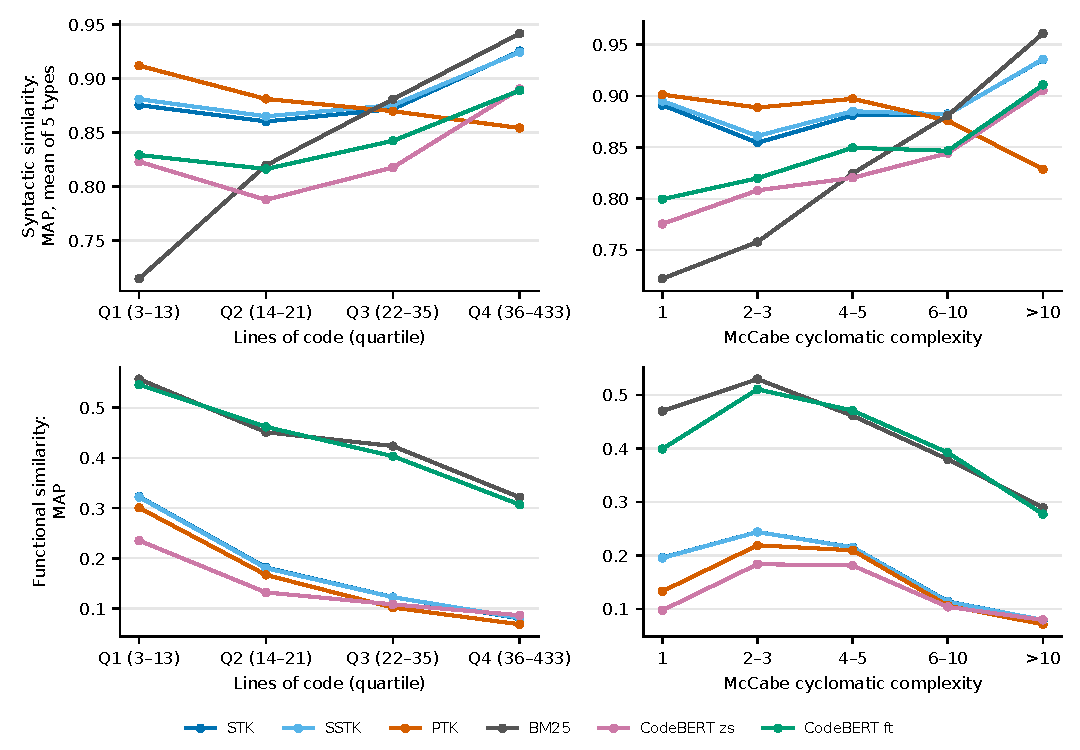
\includegraphics[width=\textwidth]{figures/rq3_size_complexity}\caption{RQ3: MAP per LOC quartile (left) and McCabe bin (right) of the query, RQ1 (top, mean of the five clone types) and RQ2 (bottom).}\label{fig:rq3}\end{figure*}

\paragraph{RQ3 groups.} Lines of code = physical lines of the method; McCabe = cyclomatic complexity (Checkstyle
10.21.1, default counting). Queries are grouped into the quartiles of lines of code over the
eligible queries (3--13, 14--21, 22--35, 36--433) and into McCabe bins 1, 2--3, 4--5, 6--10, $>$ 10, the last being
McCabe's own threshold. Candidates are not restricted by group.


\rqsection{RQ4. Hybrid: BM25 followed by a tree kernel}{How much of the tree kernels' effectiveness remains, and at what cost, when they only re-rank BM25's top 100 candidates?}
\addresses{R2-C5, R1-C1a.}
\begin{table*}[!htbp]
\centering
\caption{RQ4: hybrids (BM25's top 100 re-ranked by the kernel) next to each kernel's full ranking, BM25 and fine-tuned CodeBERT, every eligible query. Syntactic similarity: mean of the five clone types. Time: mean seconds per query over the timing sample of Table~\ref{tab:rq2}, one thread; a hybrid's time is BM25's time plus the kernel's re-ranking of BM25's top 100. $^{\ast}$/$^{\circ}$: hybrid significantly better/worse than its kernel's full ranking; $^{+}$/$^{-}$: than BM25; $^{\uparrow}$/$^{\downarrow}$: than fine-tuned CodeBERT (MAP; Bonferroni-adjusted CI excludes 0, Figure~\ref{fig:rq4}).}
\label{tab:rq4}
\footnotesize
\setlength{\tabcolsep}{3.5pt}
\begin{tabular}{lcccccccc||r}
\toprule
 & \multicolumn{4}{c}{Syntactic similarity: mean of the five types} & \multicolumn{4}{c}{Functional similarity} & \\
\cmidrule(lr){2-5}\cmidrule(lr){6-9}
Method & nP@5 & nP@10 & MRR & MAP & nP@5 & nP@10 & MRR & MAP & Time (s) \\
\midrule
STK & 0.910 & 0.909 & 0.932 & 0.876 & 0.657 & 0.600 & 0.821 & 0.183 & 6.73 \\
STK-Hybrid & 0.877 & 0.870 & 0.909 & 0.837$^{+}$ & 0.741 & 0.704 & 0.874 & 0.440$^{\ast}$ & 0.770 \\
\midrule
SSTK & 0.914 & 0.912 & 0.934 & 0.879 & 0.654 & 0.600 & 0.820 & 0.182 & 6.98 \\
SSTK-Hybrid & 0.878 & 0.870 & 0.909 & 0.838$^{+}$ & 0.740 & 0.703 & 0.874 & 0.440$^{\ast}$ & 0.767 \\
\midrule
PTK & \textbf{0.916} & \textbf{0.916} & \textbf{0.937} & \textbf{0.887} & 0.617 & 0.562 & 0.789 & 0.165 & 15.51 \\
PTK-Hybrid & 0.880 & 0.872 & 0.912 & 0.838$^{+}$ & 0.752 & 0.720 & \textbf{0.875} & 0.442$^{\ast}$ & 0.793 \\
\midrule
BM25 & 0.842 & 0.847 & 0.868 & 0.808 & 0.743 & 0.704 & \textbf{0.875} & \textbf{0.443} & 0.70 \\
CodeBERT ft & 0.873 & 0.876 & 0.894 & 0.839 & \textbf{0.753} & \textbf{0.724} & 0.868 & 0.434 & 0.41 \\
\bottomrule
\end{tabular}
\end{table*}

\begin{figure*}[!htbp]\centering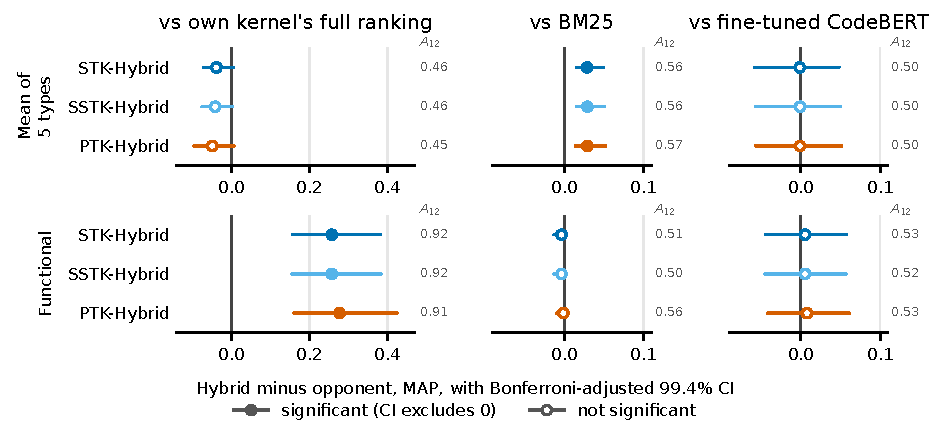
\includegraphics[width=0.87\textwidth]{figures/rq4_forest}\caption{RQ4 tests on MAP: each hybrid minus its kernel's full ranking, BM25 and fine-tuned CodeBERT, with Bonferroni-adjusted 99.4\% CI (9 comparisons per measure). Filled: the CI excludes 0. Right of each panel: effect size $A_{12}$.}\label{fig:rq4}\end{figure*}


%What the draft shows (MAP)
%- Mean of types: every hybrid beats BM25. None differs significantly from its kernel's full ranking or from fine-tuned CodeBERT.
%- RQ2: every hybrid is far above its kernel's full ranking (about +0.26), and none differs significantly from BM25 or fine-tuned CodeBERT.
%- Layout: one row per hybrid, with squares for top 100 and diamonds for top 200. Each column is one opponent, and the x-axis in the first column is wider because of those large RQ2 gains.


\end{document}
